% Author: Till Tantau
% Source: The PGF/TikZ manual

\documentclass{article}

\usepackage{pgf}
\usepackage{tikz}
\usetikzlibrary{arrows,automata}
\usepackage[latin1]{inputenc}
\usepackage{verbatim}

\begin{document}

\begin{comment}
:Title: State machine
:Tags: Manual, Automata, Graphs

Another examle from the manual.

| Author: Till Tantau
| Source: The PGF/TikZ manual

\end{comment}

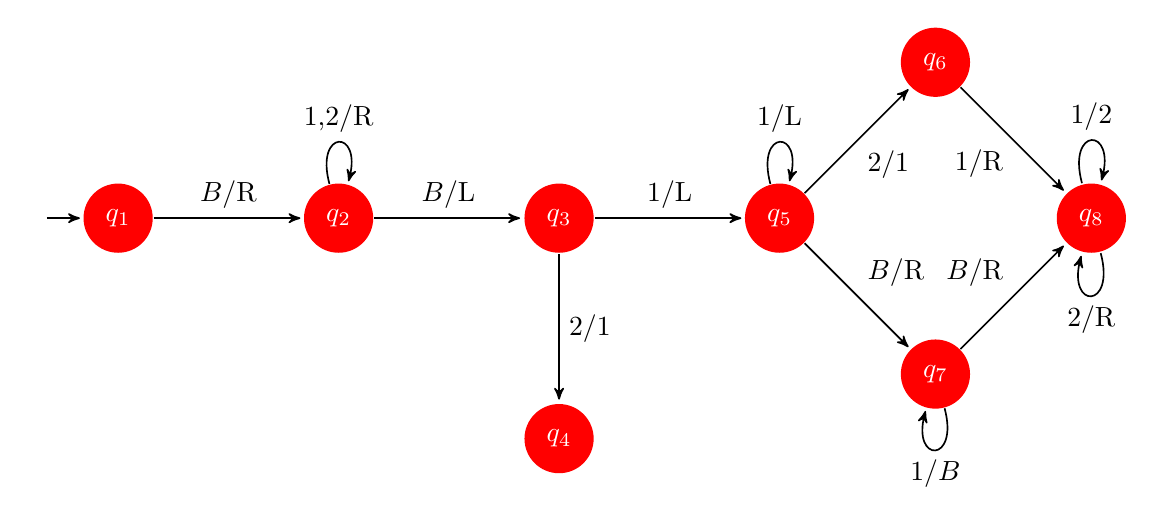
\begin{tikzpicture}[->,>=stealth',shorten >=1pt,auto,node distance=2.8cm,
                    semithick]
  \tikzstyle{every state}=[fill=red,draw=none,text=white]

  \node[state,initial,initial text={}] (q1) {$q_1$};
  \node[state] (q2) [right of = q1] {$q_2$};
  \node[state,accepting] (q3) [right of = q2] {$q_3$};
  \node[state,accepting] (q4) [below of = q3] {$q_4$};
  \node[state] (q5) [right of = q3] {$q_5$};
  \node[state] (q6) [above right of = q5] {$q_6$};
  \node[state] (q7) [below right of = q5] {$q_7$};
  \node[state,accepting] (q8) [below right of = q6] {$q_8$};

  \path (q1) edge node{$B$/R} (q2)
       (q2) edge[loop above] node{1,2/R} ()
       (q2) edge node{$B$/L} (q3)
       (q3) edge node{2/1} (q4)
       (q3) edge node{1/L} (q5)
       (q5) edge[loop above] node{1/L} ()
       (q5) edge[swap] node{2/1} (q6)
       (q5) edge node{$B$/R} (q7)
       (q6) edge[swap] node{1/R} (q8)
       (q7) edge[loop below] node{1/$B$} ()
       (q7) edge node{$B$/R} (q8)
       (q8) edge[loop above] node{1/2} ()
       (q8) edge[loop below] node{2/R} ();
\end{tikzpicture}

\end{document}
